\section{Contraintes fonctionnelles satisfaites par le logiciel}
Afin de pouvoir utiliser simplement MiniJAJA, notre application dispose d'un mini-IDE qui permet d'écrire du MiniJAJA, de le compiler en jajacode, mais aussi d'interpréter ces deux langages, ainsi que de les déboguer.

Ce mini-IDE dispose de deux thèmes de couleurs : un thème clair et un thème sombre.

\begin{figure}[h]
    \centering
    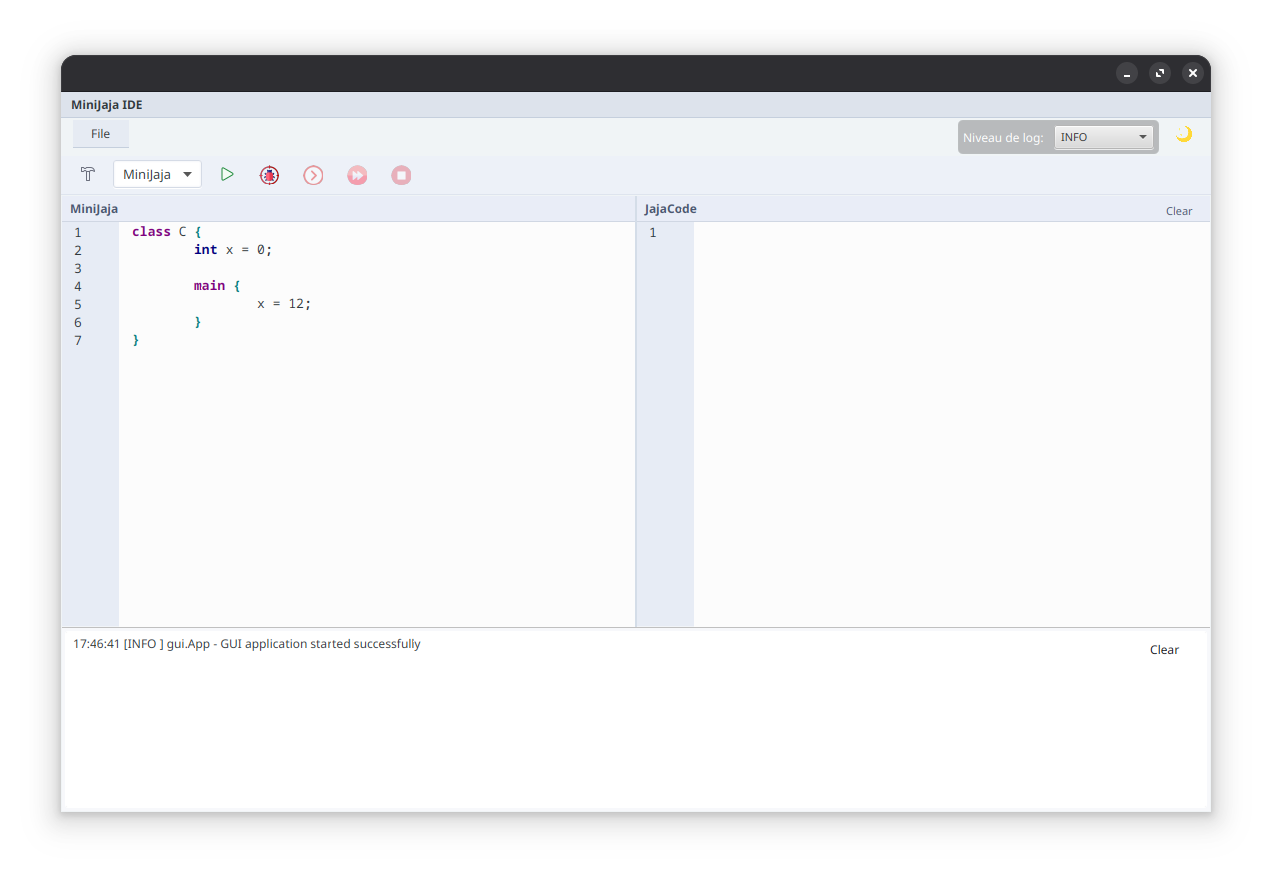
\includegraphics[width=0.4\linewidth]{images/contraintes_fonctionnelles/light.png}
    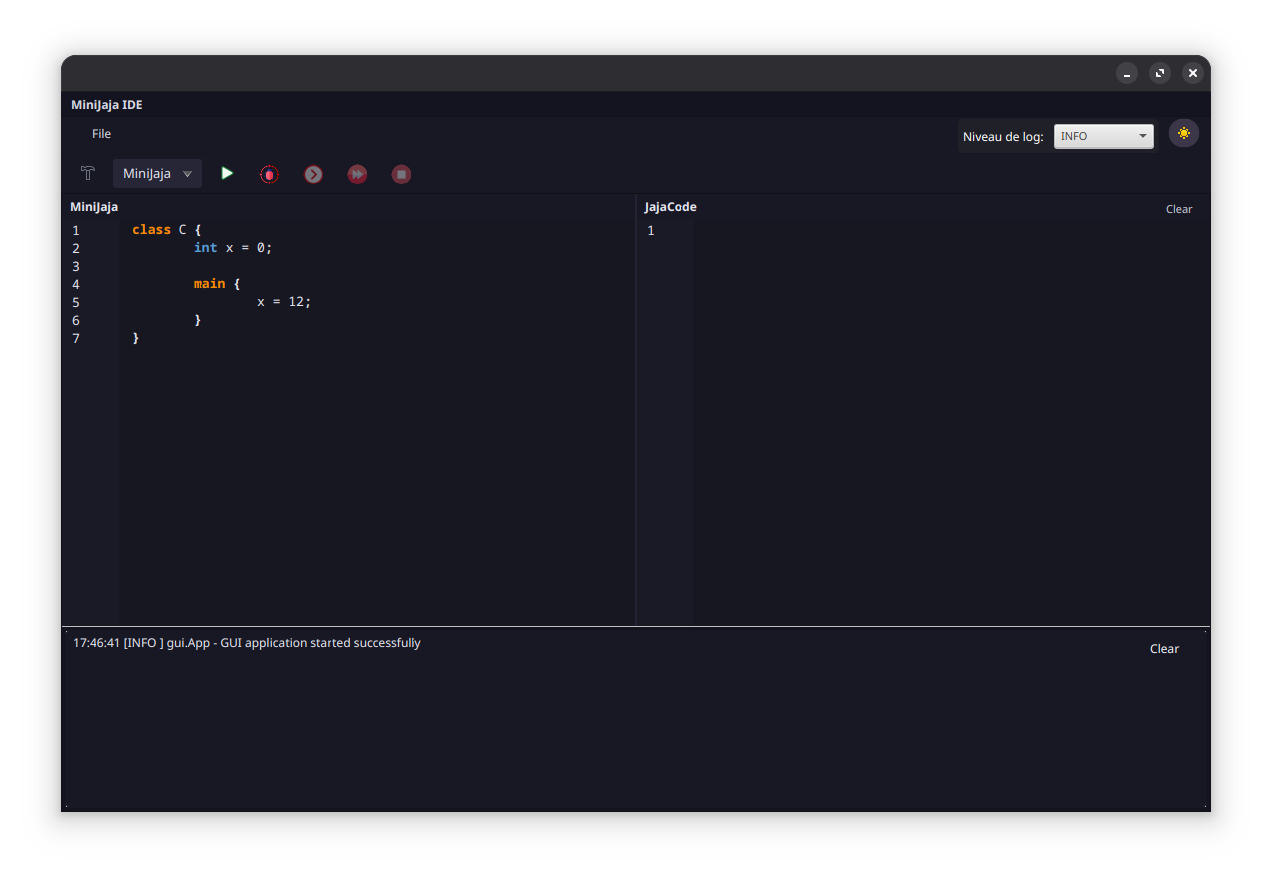
\includegraphics[width=0.4\linewidth]{images/contraintes_fonctionnelles/dark.png}
    \caption{Thème clair et sombre de notre interface}
    \label{fig:placeholder}
\end{figure}

\subsection{Écriture de fichier minijaja}
Dans cette interface, la zone centrale permet d'écrire du MiniJAJA (à gauche) et d'afficher le résultat de la compilation en jajacode (à droite).

Pour nous aider lors de l'écriture de programmes MiniJAJA, notre interface propose la complétion automatique, la coloration syntaxique ainsi que la numérotation des lignes.

Il est également possible d'ouvrir et de sauvegarder des fichiers.
\begin{figure}[h]
    \begin{minipage}{.6\textwidth}
        \centering
        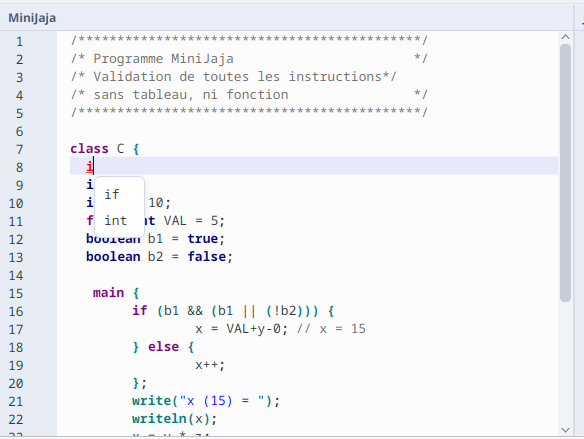
\includegraphics[width=0.7\linewidth]{images/contraintes_fonctionnelles/minijaja_area.png}
        \captionof{figure}{Exemple d'écriture de code miniJAJA}
        \label{fig:placeholder}
    \end{minipage}%
    \begin{minipage}{.3\textwidth}
        \centering
        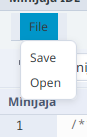
\includegraphics[width=0.5\linewidth]{images/contraintes_fonctionnelles/open_and_save.png}
        \captionof{figure}{Ouverture et sauvegarde de fichiers}
        \label{fig:placeholder}
    \end{minipage}
\end{figure}


\subsection{Compilation et interprétation}
Notre interface permet de compiler du MiniJAJA en jajacode grâce au premier bouton de la barre d'outils. Lors de la compilation du MiniJAJA, le jajacode obtenu apparaît dans la partie droite de l'interface.

\begin{figure}[h]
    \centering
    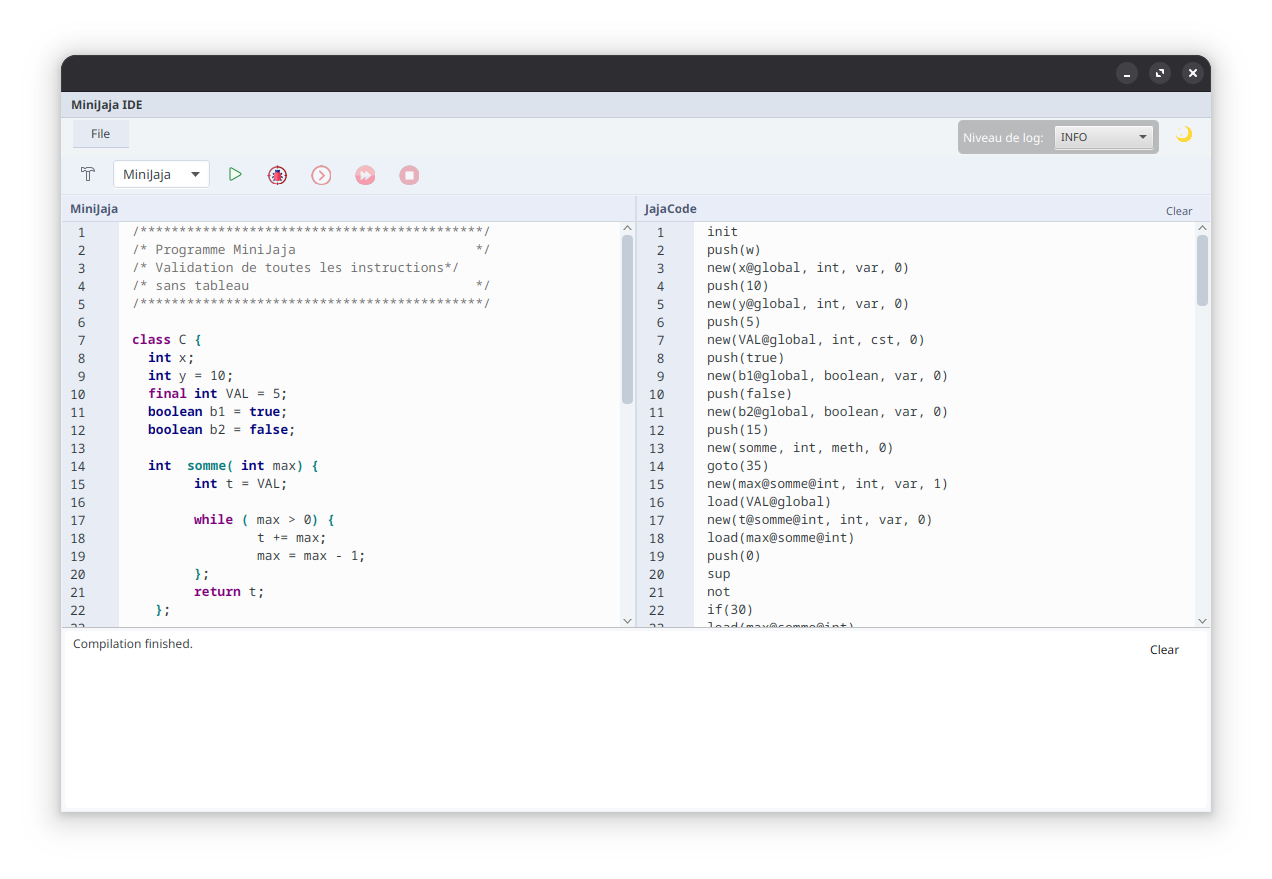
\includegraphics[width=0.8\linewidth]{images/contraintes_fonctionnelles/compile.png}
    \caption{Interface après compilation}
    \label{fig:placeholder}
\end{figure}

Le deuxième bouton de l'interface permet d'interpréter le MiniJAJA ou le jajacode en fonction de l'élément sélectionné dans la liste déroulante située juste avant (cette liste permet également de choisir quel code déboguer).

Lorsque l'on compile ou interprète du code, on obtient plus ou moins d'informations dans la console en fonction du niveau de logs choisi.

\subsection{Débogage}
Pour passer en mode débogage, il suffit de choisir le code à déboguer grâce à la liste déroulante, puis de cliquer sur le bouton « bug » situé à côté du bouton permettant de démarrer l'interprétation.

Une fois le mode débogage démarré, plusieurs options s'offrent à nous :
\begin{itemize}
    \item Soit aucun point d'arrêt (breakpoint) n'est placé dans l'interface ; dans ce cas, le débogage se fait pas à pas et le débogueur s'arrête à la première ligne de code.
    \item Soit des points d'arrêt sont positionnés et le débogueur s'arrête au premier point d'arrêt rencontré.
\end{itemize}

Ensuite, il est possible de reprendre le débogage pas à pas à l'aide de la simple flèche, ou de reprendre l'exécution jusqu'au prochain point d'arrêt avec la double flèche.

 \begin{figure}[h]
     \centering
     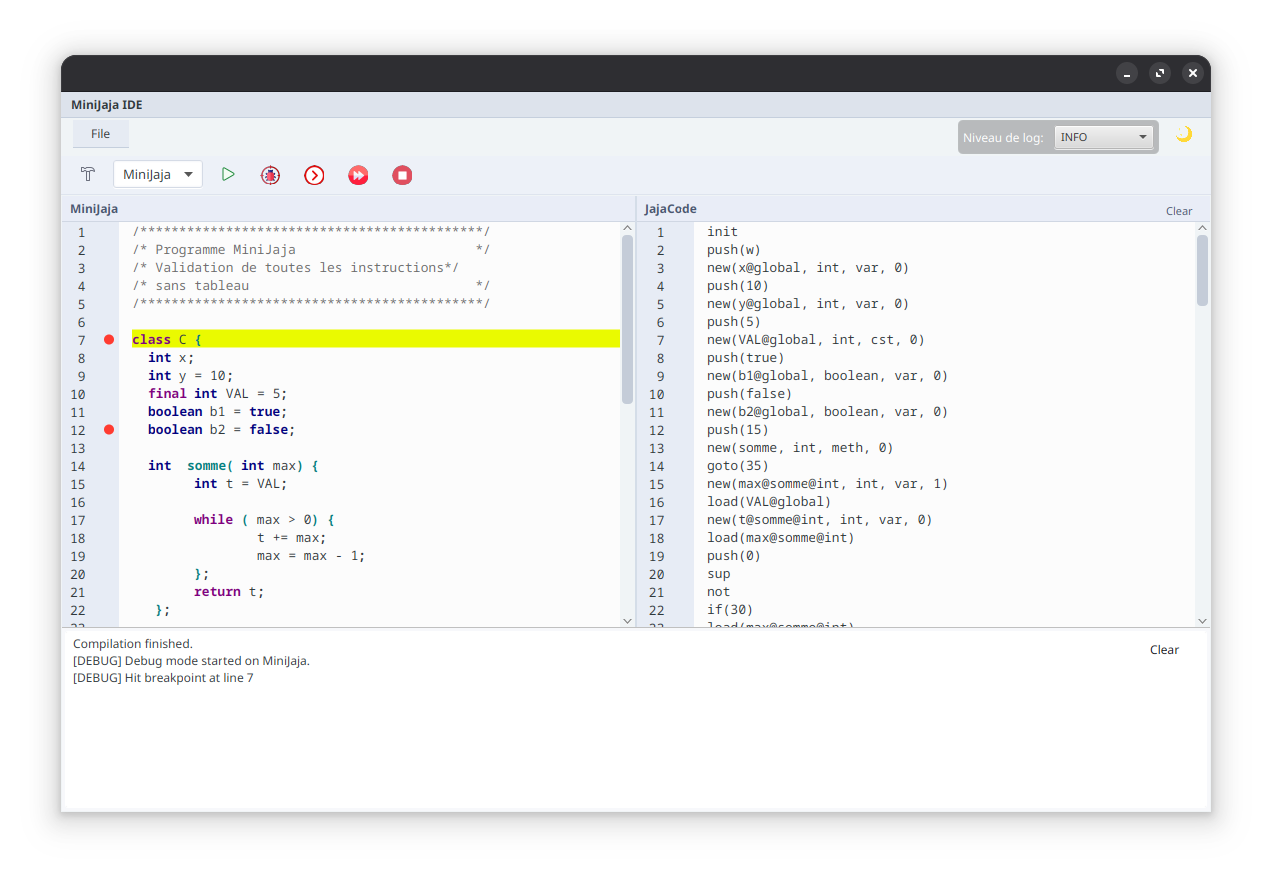
\includegraphics[width=0.8\linewidth]{images/contraintes_fonctionnelles/debuging.png}
     \caption{Exemple d'utilisation du mode débogue}
     \label{fig:placeholder}
 \end{figure}

Un affichage de la mémoire à côté de la console est en cours de préparation afin de pouvoir observer les changements de la mémoire au cours du débogage.

\begin{figure}
    \centering
    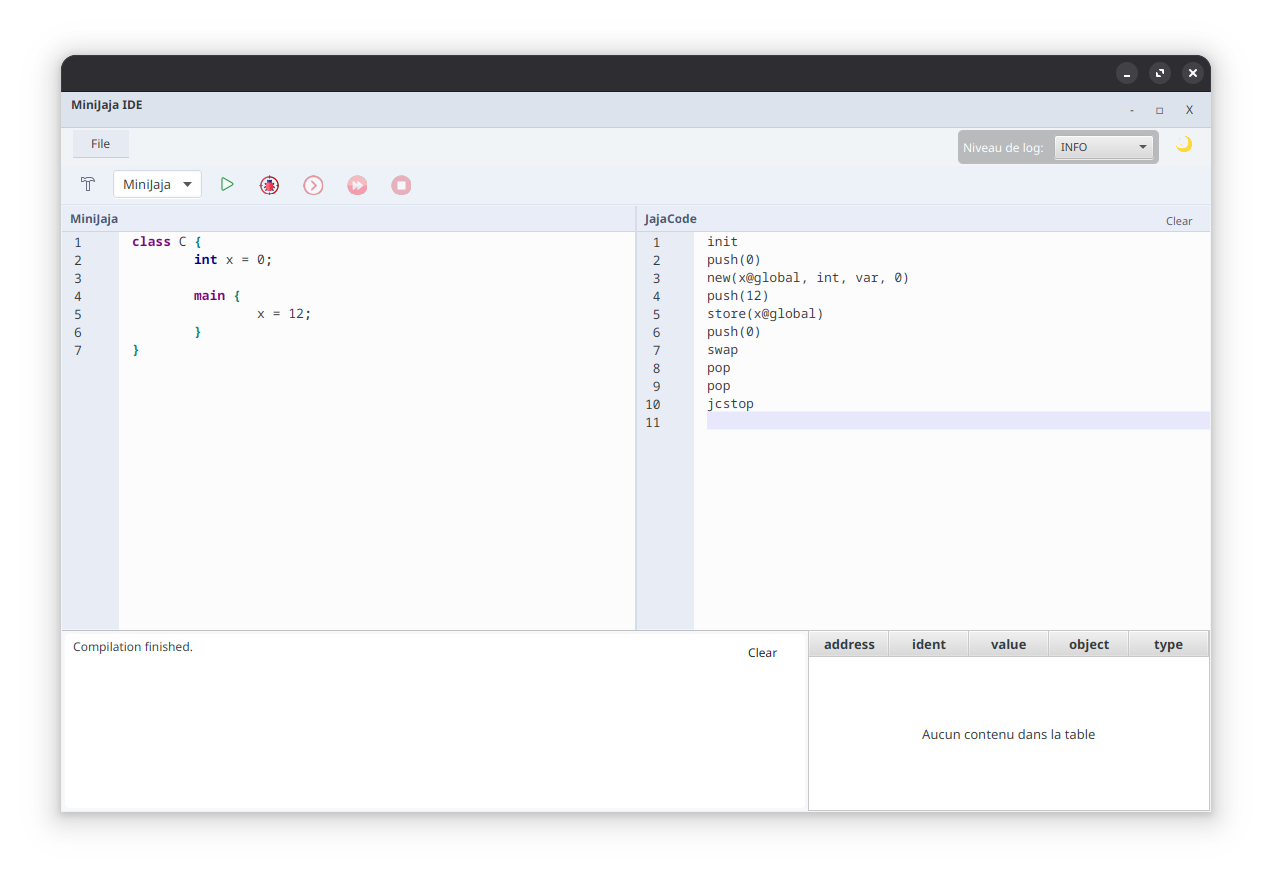
\includegraphics[width=0.8\linewidth]{images/contraintes_fonctionnelles/memoire.png}
    \caption{Affichage de la mémoire pendant le déboguage}
    \label{fig:placeholder}
\end{figure}
